\documentclass[conference]{IEEEtran}
\usepackage{kotex}
\linespread{1.35}
\usepackage{cuted}
\usepackage{color}
\usepackage{caption}
\usepackage{listings}
\usepackage{tcolorbox}
\usepackage{graphicx}
\usepackage{subcaption}
\usepackage{hyperref}

\lstset{
  label=DescriptiveLabel,
  language=Python,
  caption={match score function},
  keywordstyle=\color{blue},       % keyword style
  frame=top,frame=bottom,
  basicstyle=\small\normalfont\sffamily,    % the size of the fonts that are used for the code
  stepnumber=1,                           % the step between two line-numbers. If it is 1 each line will be numbered
  numbersep=10pt,                         % how far the line-numbers are from the code
  tabsize=2,                              % tab size in blank spaces
  extendedchars=true,                     %
  breaklines=true,                        % sets automatic line breaking
  captionpos=t,                           % sets the caption-position to top
  mathescape=true,
  stringstyle=\color{white}\ttfamily, % Farbe der String
  showspaces=false,           % Leerzeichen anzeigen ?
  showtabs=false,             % Tabs anzeigen ?
  xleftmargin=17pt,
  framexleftmargin=17pt,
  framexrightmargin=17pt,
  framexbottommargin=5pt,
  framextopmargin=5pt,
  showstringspaces=false      % Leerzeichen in Strings anzeigen ?
 }

\DeclareCaptionFormat{listing}{\rule{\dimexpr\textwidth+17pt\relax}{0.4pt}\par\vskip1pt#1#2#3}
\captionsetup[lstlisting]{format=listing, singlelinecheck=false, margin=0pt, labelsep=space,labelfont=bf}

\renewcommand\lstlistingname{Code}
\hypersetup{
    colorlinks=true,
    linkcolor=blue,
    filecolor=magenta,      
    urlcolor=cyan,
}

\IEEEoverridecommandlockouts

% The preceding line is only needed to identify funding in the first footnote. If that is unneeded, please comment it out.
\usepackage{cite}
\usepackage{amsmath,amssymb,amsfonts}
\usepackage{algorithmic}
\usepackage{graphicx}
\usepackage{textcomp}
\usepackage{xcolor}
\def\BibTeX{{\rm B\kern-.05em{\sc i\kern-.025em b}\kern-.08em
    T\kern-.1667em\lower.7ex\hbox{E}\kern-.125emX}}
    
\begin{document}

\title{
{\footnotesize 2024학년도 1학기 빅데이터분석 \\}
질병-증상 데이터를 활용한 ARM 기반\\증상에 따른 질병 예측 시스템\\
}

\author{김채원 \\
지능전자컴퓨터공학과 248251}

\maketitle

\section{Introduction}
본 문서는 질병-증상 데이터를 크롤링하고, 이를 기반으로 association rule mining (ARM)을 수행하여 사용자의 증상에 따른 질병을 예측하는 시스템 구축에 대한 결과보고서이다. 사용자가 입력한 증상을 분석하여 가장 가능성이 높은 질환을 반환하며, 이를 통해 사용자는 내원하지 않고 적은 비용으로 자신의 증상에 대한 질환을 탐색할 수 있도록 한다.

\section{Materials and Methods}

\subsection{Data Collection}
정보를 수집하고자 하는 질환 20개를 선정하였다. 이때 급성 질환이거나 일상에서 자주 보이는 익숙한 질환을 주로 선정하였다.
\begin{itemize}
    \item 과민성 대장 증후군, 당뇨병, 심부전, 천식, 급성 대장염, 감기, 급성 경막하 출혈, 인플루엔자, 긴장성 두통, 고산병, 아나필락시스, 루게릭병, 장폐색, 아토피 피부염, 대상포진, 돌발성 난청, 만성 비염, 급성 신우신염, 뇌전증, 패혈증
\end{itemize}

Selenium을 활용하여 서울대학교 병원과 서울아산병원 홈페이지에서 질병-증상 데이터를 크롤링하였다. 질환명 검색 결과 페이지에서, 검색한 질환명과 게시물 제목 모두 띄어쓰기를 제거하고 1) 완전 일치하는지, 2) 포함관계인지 확인했다. 서울대학교 병원에서는 질환 정보 게시물 제목에 \verb|[N의학정보]|라는 태그를 사용하고 있어, 질환을 검색한 결과 페이지에서 제목 HTML 요소에 \verb|[N의학정보]| 태그가 포함되어 있는 게시물을 우선 탐색하였다. 서울대학교 병원에서는 질환의 국문명, 질환의 영문명, 관련 증상(증상 키워드), 정의, 증상, 원인, 진단, 치료, 생활가이드, URL 정보를 수집하였다.

서울아산병원에서도 유사한 과정으로 질환 정보를 검색하였다. 서울아산병원에서는 질환명의 동의어도 함께 제공하고 있어 검색 질환과 게시물의 일치 여부를 게시물의 제목 뿐만 아니라 동의어 목록에서도 확인했다. 또한 질환의 국문명으로 검색 시에 게시물이 존재하지 않는 경우도 있었는데, 이때는 앞서 서울대학교 병원 홈페이지에서 수집한 질환의 영문명으로 검색하여 문제를 해결하였다. 서울 아산병원에서는 질환의 국문명, 질환의 영문명, 동의어, 증상 키워드, 정의, 증상, 원인, 진단, 치료, 경과, 주의사항, URL 정보를 수집했다.

\subsection{Data Preprocessing}
두 병원에서 수집한 데이터를 병합하였다. 증상 키워드 컬럼은 키워드의 등장 빈도수를 고려하기 위해 병합 시 중복 제거를 수행하지 않았다. 또한, 각 데이터에 질환의 증상이 서술되어 있는 증상 컬럼이 존재했는데, \verb|Konlpy| 라이브러리를 사용하여 명사만 추출하였다. 이 명사들 중 증상 키워드 컬럼에 존재하는 명사만 증상 키워드 컬럼에 추가해주었다. 즉, 증상 키워드 컬럼에는 서울대학교 병원과 서울아산병원의 증상 키워드 데이터, 증상 컬럼에서 추출 및 필터링한 명사 데이터가 포함되어 있다.

다음으로 동의어 처리를 수행했다. 두 개의 홈페이지에서 수집한 데이터이므로 \{``발열": ``열"\}, \{``어지럼증": ``어지러움"\} 등 동의어가 혼재했다. 따라서 용어 통일이 필요했다. 이는 자동화가 어려워 전체 증상 키워드에서 통일할 단어를 직접 선정했다. 그 후 각 증상 키워드가 해당 질환에서 몇 번 등장하였는지 빈도를 확인하여 \verb|key|가 증상 키워드, \verb|value|가 빈도 수인 \verb|dictionary| 형태로 저장했다.

\subsection{Apriori Algorithm \& Association Rule Mining (ARM)}
증상 키워드 컬럼에 등장하는 모든 고유한 단어 107개를 기반으로 transaction table을 구성한다. 그리고 Apriori algorithm을 적용하여 item set의 수를 줄인다. \verb|min_support|는 0.1로 설정했다. Apriori algorithm은 A가 B의 부분집합이라면, A의 support는 B의 support보다 크거나 같다는 아이디어를 바탕으로 한다. 따라서 B의 support가 \verb|min_support|보다 크면 A의 support 또한 \verb|min_support|보다 크다. 이를 바탕으로 support가 \verb|min_support|보다 큰 item set을 추린다.
Apriori algorithm을 통해 얻은 item set을 기반으로 ARM을 수행한다. 생성된 규칙을 \verb|confidence| 기준으로 내림차순 정렬한다.

\subsection{Analyze user inputs \& Predict Diseases}
사용자로부터 증상 키워드를 콤마(,)로 구분하여 입력하도록 한다. 이때 입력할 수 있는 증상은 1개 이상이며, 수집한 데이터 내에 존재하는 키워드여야만 한다. 사용자가 입력한 증상 리스트로부터 모든 부분집합을 추출한다. 이를 left hand, 즉 antecedent로 갖는 모든 규칙을 필터링한다. 해당하는 규칙들의 left hand와 right hand를 병합하여 증상 리스트를 생성한다. 이 증상 리스트는 사용자가 입력한 증상과 함께 나타날 수 있는 증상들을 묶어놓은 리스트가 된다.
이제 다음 세 가지 조건에 따라 질환을 추린다.
\begin{enumerate}
    \item ``사용자의 증상"과 ``질환의 증상 키워드"가 완전 일치하는 질환
    \item ``ARM 기반 증상 리스트"가 ``질환의 증상 키워드"의 부분집합인 질환
    \item ``사용자의 증상"이 ``질환의 증상 키워드"의 부분집합인 질환
\end{enumerate}
추려낸 각 질환의 증상과 사용자의 증상 간 score를 구한다 (Code \ref{DescriptiveLabel}). Score를 기준으로 질환을 내림차순 정렬하고, 상위 3개의 질환만을 출력한다. 출력되는 정보는 질환의 순위, 질환명, 증상과 증상의 빈도 수, score, 서울대학교 병원과 서울아산병원의 URL이다.
\subsection{Provide life guide information}
질환을 예방하거나 증상을 완화하기 위해 사용자가 일상생활에서 실천할 수 있는 생활 가이드 정보를 제공한다. 사용자가 질환명을 입력하면, 해당 질환에 대한 생활 가이드, 주의사항, 예방방법 정보를 출력한다. 이때, 사용자가 검색한 질환이 앞서 예측한 3개의 질환에 포함되지 않는다면 "해당 질환은 입력하신 증상과 일치할 확률이 낮습니다."라는 메시지를 출력한다. 또한, 해당 질환이 내원을 요구하는 응급 질환인 경우에도 관련 메시지를 출력하도록 구현했다.
\begin{strip}
\begin{lstlisting}[label=DescriptiveLabel, frame=tb, escapeinside=``, language=Python]
def match_score(disease):
    score = 0    `\# 총 점수`
    count = 0    `\# 질환의 증상에 사용자의 증상이 몇 개나 포함되는지`
    for i in range(len(df)):
        if df["`질환명`"][i] == disease:
            symp_dict = eval(df["`증상 등장 빈도`"][i])[0]    `\# 질환의 {증상: 빈도수} 딕셔너리`
            for symptom in user_symptoms:    `\# 사용자의 증상들`
                if symptom in symp_dict.keys():    `\# 질환의 증상에 사용자의 증상이 있으면`
                    score += symp_dict[symptom]    `\# 질환의 증상 빈도수를 score에 더함`
                    count += 1    `\# 사용자의 증상이 질환의 증상에 포함되어 있으므로 count += 1`
    score = score * count    `\# 사용자의 증상이 질환의 증상에 포함되는 수만큼 score에 곱함`
\end{lstlisting}
\end{strip}


\section{Results}
Fig. \ref{fig:1}에서 사용자가 ``두통", ``어지럼증", ``호흡곤란"을 입력하면, score를 기준으로 내림차순 정렬한 질환들과 상위 3개 질환의 상세정보를 출력한다. 사용자의 입력이 모두 포함되어 있는 질환인 ``고산병"이  1순위 질환으로 선정됐다. 2순위와 3순위 질환은 모두 ``두통", ``호흡곤란"을 포함하고 있는데, ``급성 경막하 출혈"에서는 ``두통"이 5회, ``호흡곤란"이 2회 등장했고 ``심부전"에서는 각 2회 등장하여 ``급성 경막하 출혈"의 score가 더 높아 2순위 질환으로 선정됐다.

또한 생활 가이드 정보를 얻기 위해 ``아나필락시스"를 입력하자 일상생활에서 실천 가능한 정보와 함께 내원 안내 메시지가 출력되는 것을 볼 수 있다.
\begin{figure*}
\centerline{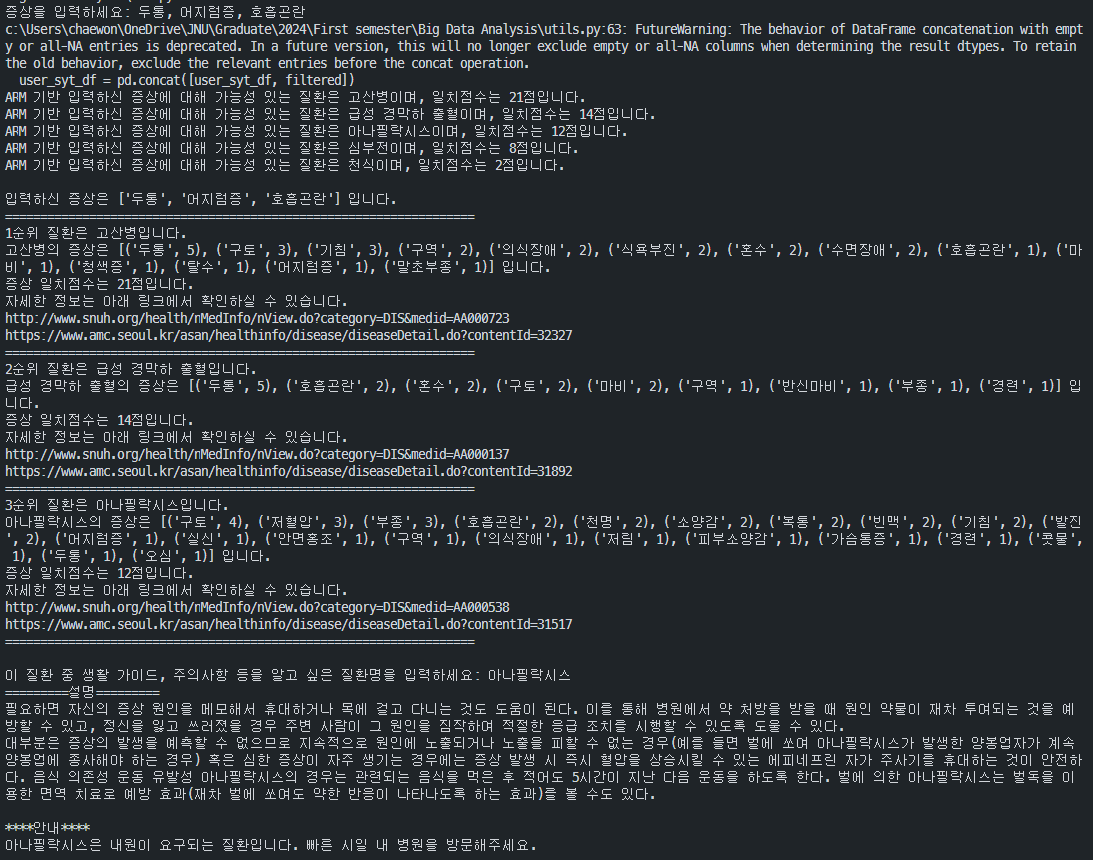
\includegraphics[width=0.95\textwidth]{temp.png}}
\caption{Total results}
\label{fig:1}
\end{figure*}

또다른 예시인 Fig. \ref{fig:2}에서는 사용자가 입력한 증상에 따라 예측되는 질환이 달라지는 결과를 보여준다. Fig. \ref{fig:2a}에서 사용자 입력 증상은 ``오한", ``열"이며, 예측된 질환은 ``인플루엔자", ``급성 신우신염", ``패혈증"이다. 여기에 ``기침" 증상을 추가로 입력해주면 예측 질환은 ``인플루엔자", ``감기", ``급성 신우신염"으로 바뀐다 (Fig. \ref{fig:2b}). 즉, ``기침" 증상이 나타나는 질환인 ``감기"의 score가 높아지면서 상위 질환의 순서가 변경된 것이다. 이를 통해 score 계산 기준이 본 프로젝트의 목적에 부합하도록 구현되어 있음을 확인할 수 있다.

\begin{figure*}
    \centering
    \begin{subfigure}[t]{0.49\textwidth}
        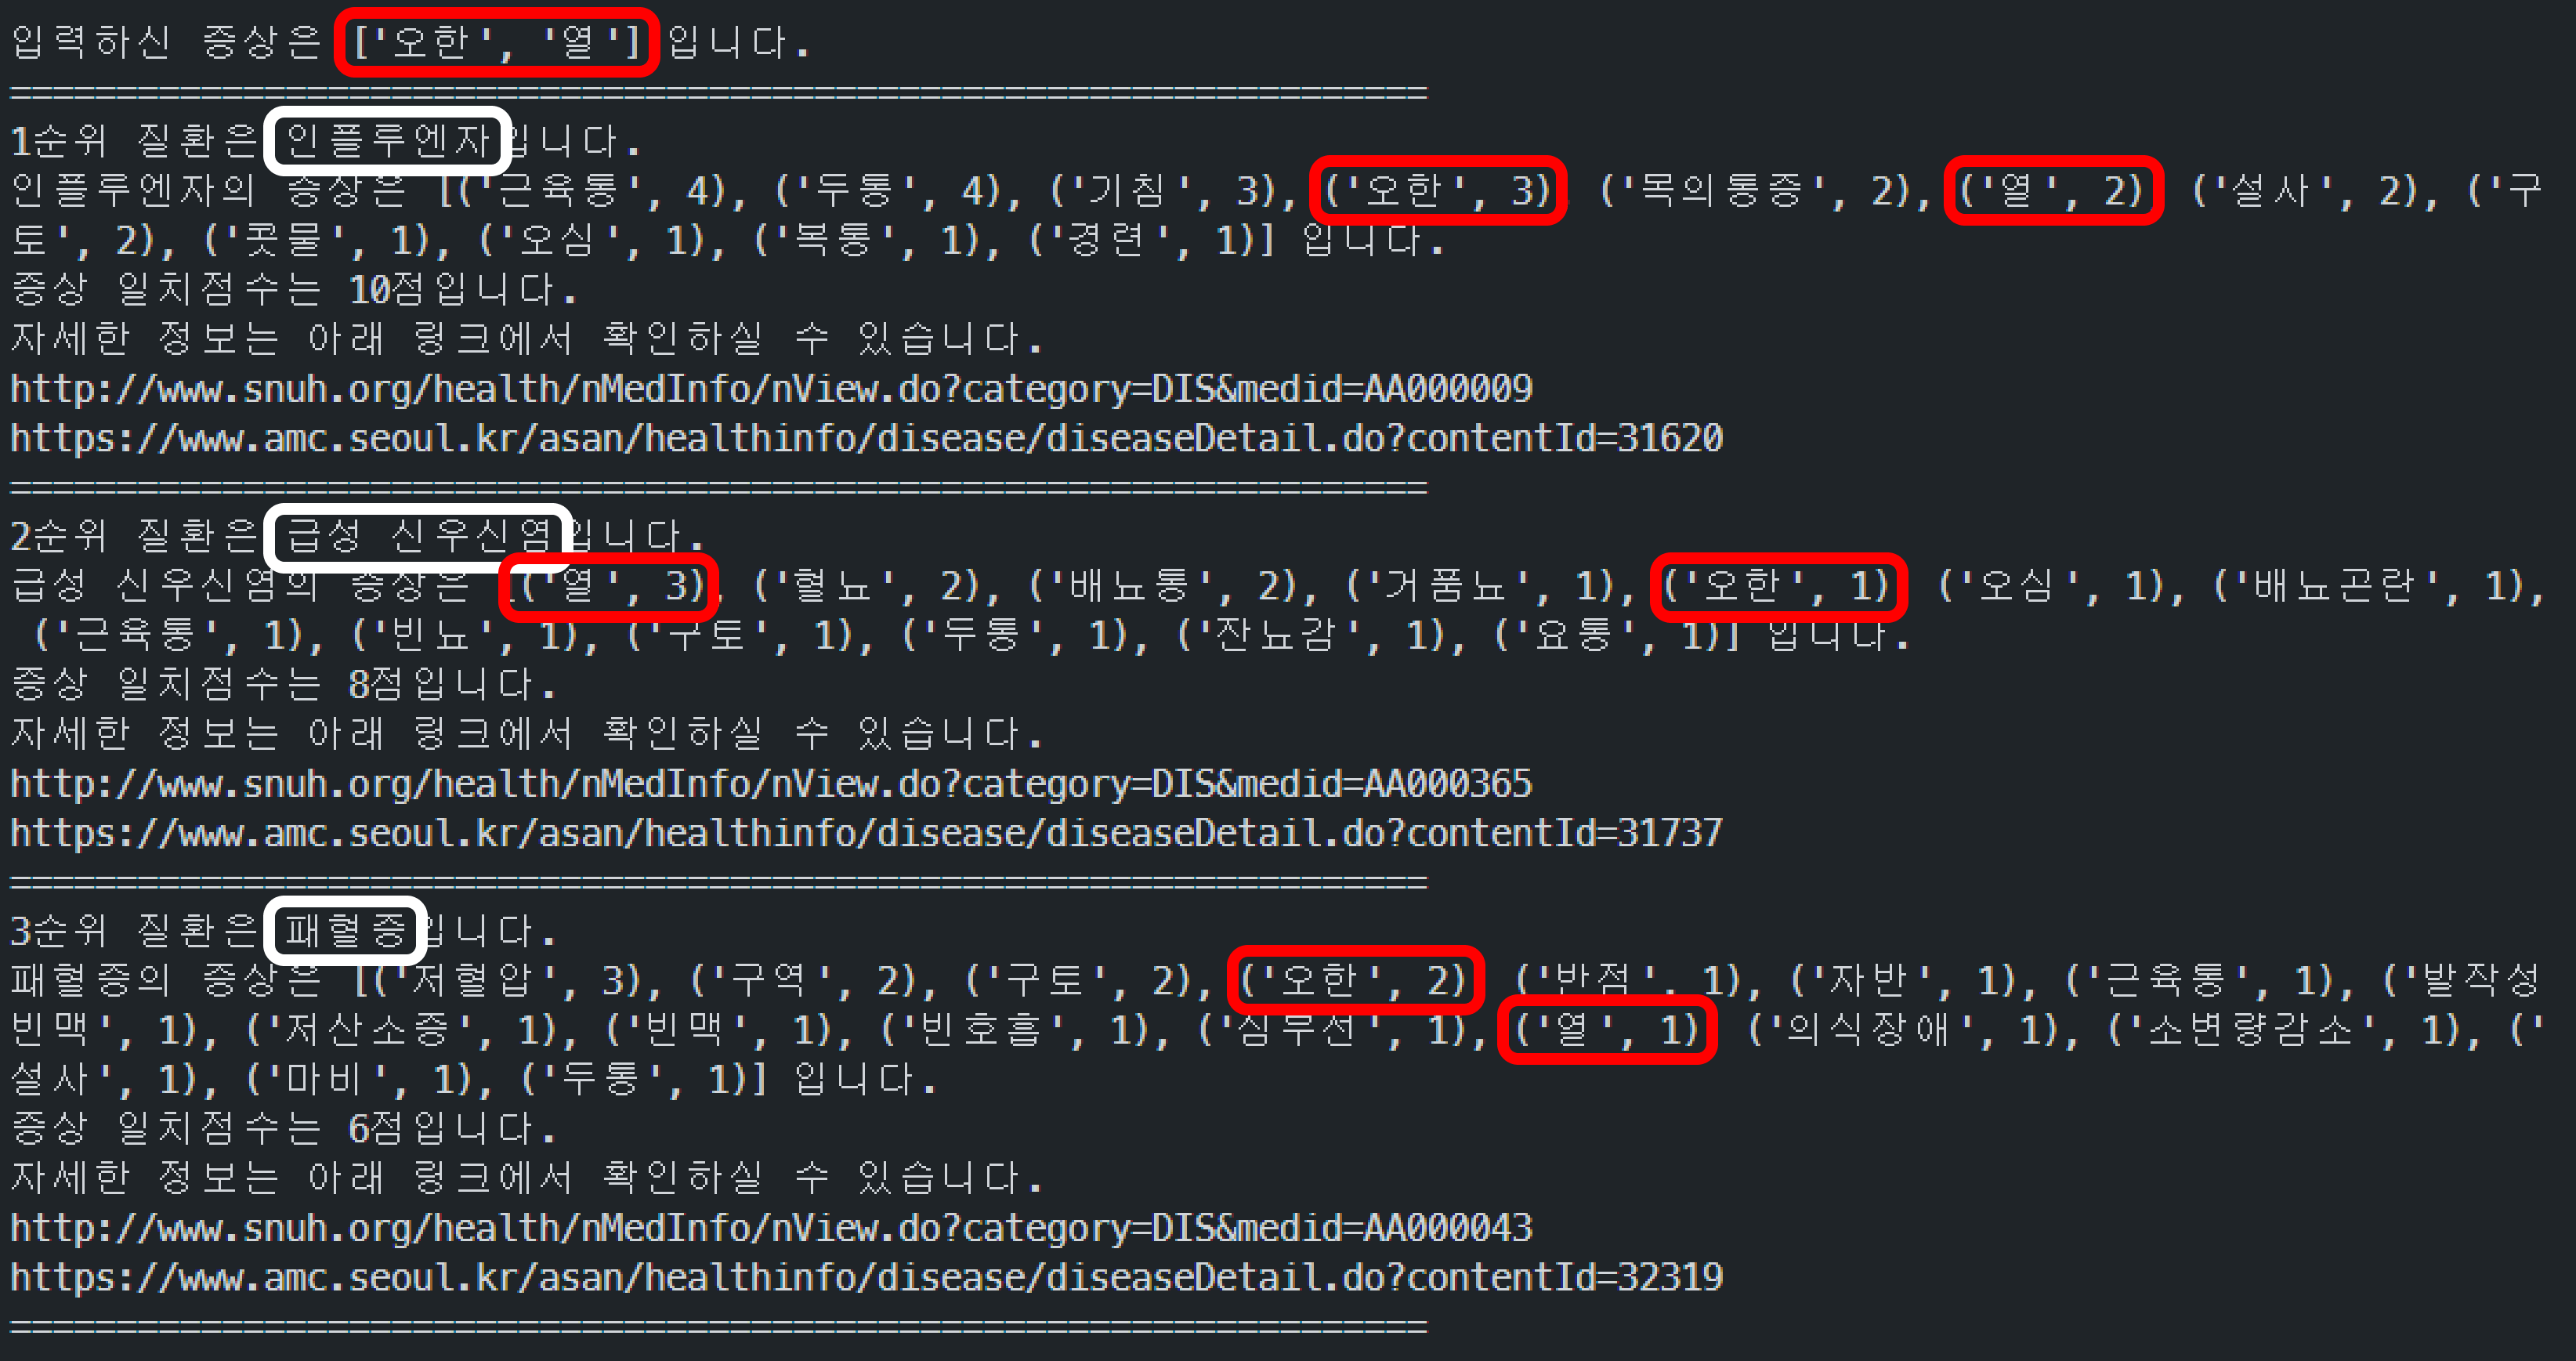
\includegraphics[width=\textwidth]{temp1.png}
        \caption{사용자 입력: ``오한", ``열"}
        \label{fig:2a}
    \end{subfigure}
    ~ %add desired spacing between images, e. g. ~, \quad, \qquad, \hfill etc. 
      %(or a blank line to force the subfigure onto a new line)
    \begin{subfigure}[t]{0.49\textwidth}
        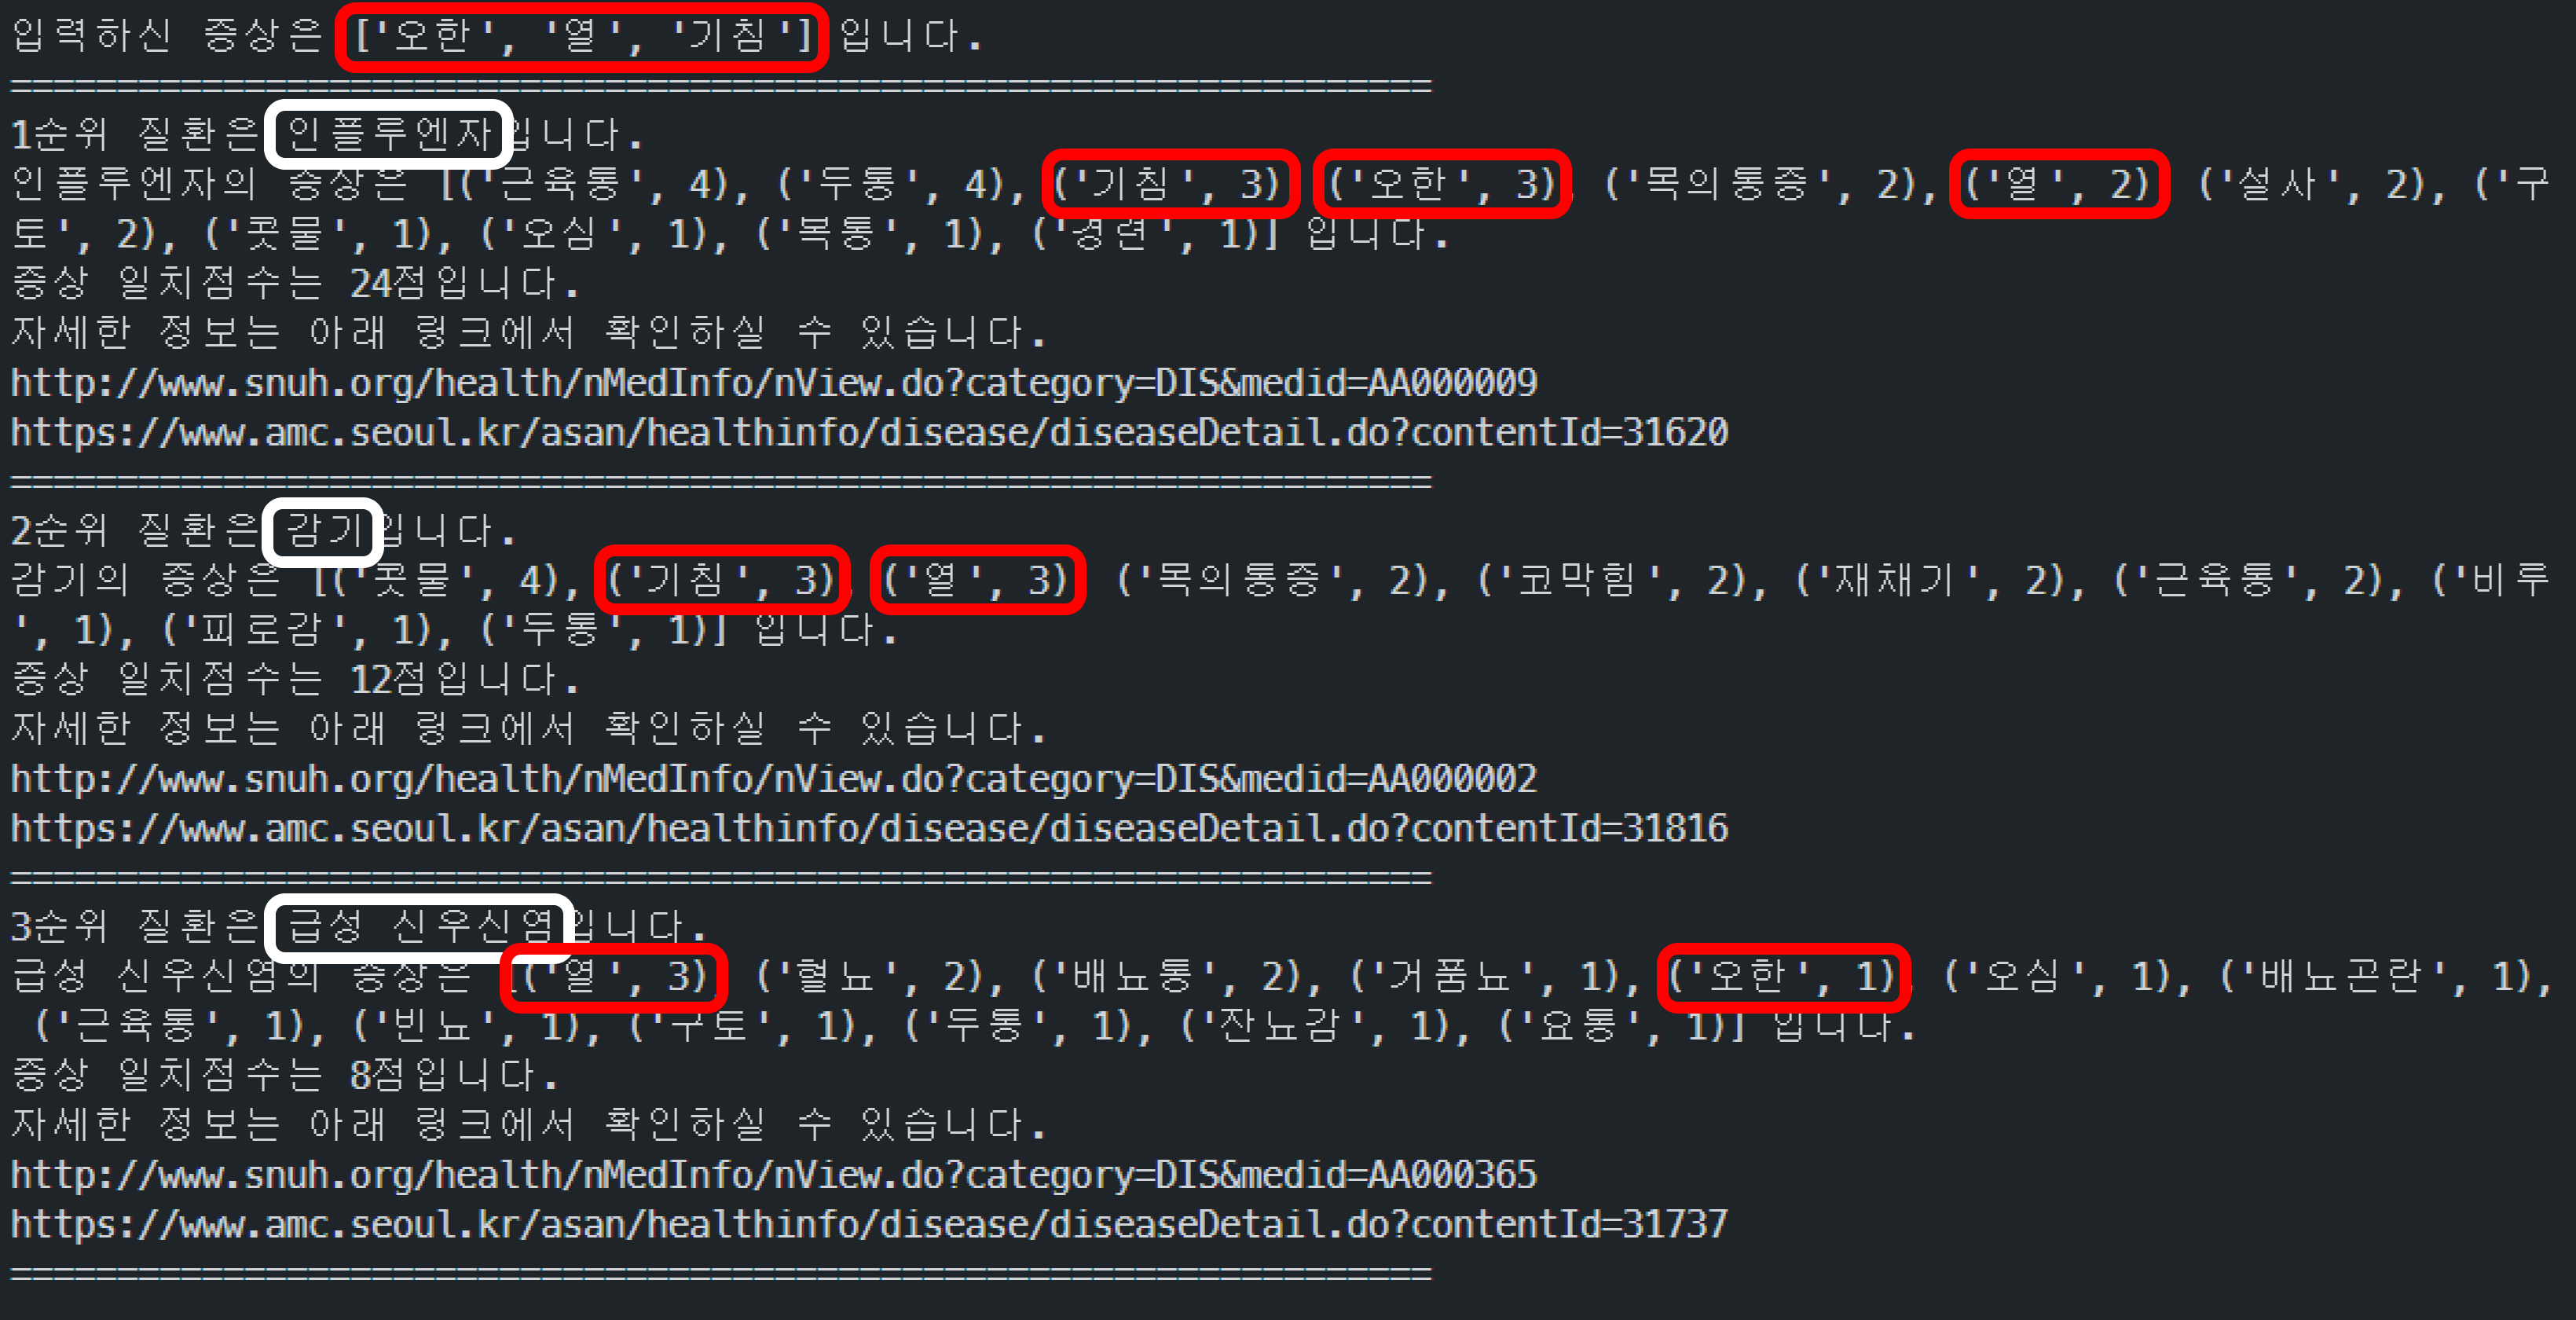
\includegraphics[width=\textwidth]{temp2.png}
        \caption{사용자 입력: ``오한", ``열", ``기침"}
        \label{fig:2b}
    \end{subfigure}
    \caption{입력 증상에 따라 다르게 예측되는 질환}\label{fig:animals}
    \label{fig:2}
\end{figure*}

\section{Conclusions}
본 프로젝트에서는 사용자의 입력 증상을 분석하고, ARM을 기반으로 가장 가능성이 높은 질환을 예측하는 시스템을 구축했다. 사용자의 증상과 가장 빈번히 함께 나타나는 증상을 탐색하고, 해당 증상들이 나타날 수 있는 질환을 출력한다. 이를 통해 사용자는 병원에 내원하지 않고 적은 비용으로 자신의 증상에 대한 질환을 확인할 수 있다.

본 시스템에는 분명한 한계도 존재한다. 첫째, 정보를 수집한 질환의 개수가 20개뿐이므로 이 데이터 셋에 포함되지 않는 증상이나 질환은 분석 및 예측할 수 없다. 둘째, 사용자가 복수의 질환을 앓고 있는 경우를 고려하지 않는다. 셋째, 사용자가 입력한 각 증상에 대한 심각도를 고려하지 않는다. 같은 증상들을 보이더라도 어떤 증상이 더 심한지에 따라 실제 진단되는 질환이 달라질 수 있으나, 이에 대한 데이터를 수집하기 어려워 고려하지 않았다.

따라서 본 시스템의 정확도와 신뢰도 향상을 위해서는 대규모의 데이터셋 구축, ARM 외 다양한 방법론 적용 등 한계점을 보완하는 후속연구가 필요할 것으로 보인다.


\section*{Changes since the midterm presentation}

중간발표 이후 변동사항은 다음과 같다.
\begin{enumerate}
    \item Score 계산식 수정
    \item 서술형 문장으로 구성된 ``증상" 컬럼에서 명사를 추출하여 분석에 추가적으로 사용
    \item 누락된 동의어 전처리 추가 수행
\end{enumerate}

\section*{Availability of data and materials}
본 프로젝트에서 수집 및 분석한 데이터와 코드는 \href{https://github.com/chaewon215/DiagnosisAssistant}{https://github.com/chaewon215/DiagnosisAssistant}에서 확인할 수 있습니다.

\end{document}